\tableofcontents
\chapter{Introduction}\label{c:Introduction}
\section{Overview of this thesis}
The study of cross-linguistic functional categories such as evidentiality, egophoricity, epistemic modality, engagement, and mirativity is a growing field in linguistics, having grown enormously over the forty years since the publication of \citeA{ChafeNichols1986} introducing evidentiality as a cross-linguistic category. This thesis provides a typological overview of these categories under the supercategory of \textsc{epistemic} marking (introduced in \ref{s:Intro:Thesis} below) within the \lfam\ language family. It uses published data and analyses of epistemic marking in 67 \lfam\ languages\footnote{A full list is given in \ref{appendix}} and original data and analysis of one language to draw up an initial typological description of this marking in the family, and in turn use these observations and trends to draw some broader theoretical conclusions about this marking both in the \lfam\ family, as well as across language more broadly.

This thesis is divided into seven chapters. This first chapter provides an overview of the thesis and its argument, as well as an overview of the literature on important and relevant ocncepts such as epistemic marking, intersubjectivity, and perspective in language. Chapter \ref{c:THOverview} gives an in-depth introduction to the \lfam\ language family, including an overview of the family itself, the current state of research and description of the family, and the history of linguistic research in the area. Chapter \ref{c:Methods} details the methodological foundations of this project, in terms of the selection of languages and data and the typological analysis of said data. It also details the methodologies of the field work undertaken to acquire supplementary data on Lhokpu (Subfamily unclear: Bhutan). Chapter \ref{c:Description} presents an initial description of epistemic marking in \lfam\ languages from the data, providing a number of typological observations in terms of the forms and functions of grammaticalised epistemic marking across the family. Chapter \ref{c:Discussion} takes these typological observations and draws more in-depth theoretical conclusions about epistemic marking both in \lfam\ languages and more generally. Chapter \ref{c:History} uses the substantial amount of typological data now collected to investigate possible pathways for the development of the widespread epistemic marking seen across the \lfam\ family in historical terms, considering both linguistic and extra-linguistic factors such as population contacts through trade or political influence. Finally, Chapter \ref{c:Conclusion} concludes this thesis with a summary of the arguments and findings presented in the earlier chapters.

Given the number of languages across the \lfam\ family discussed throughout this thesis, language names will be presented with their subfamily (as per \citeA{VanDriem2014}, see Sections \ref{ss:THOverview:Subfamilies} and \ref{ss:Methods:RepSample} for discussions on the subfamily structure of the family) along with the country in which they are spoken. In cases where a language is not clearly a member of a wider subfamily, it is labelled as either \textit{Internal isolate} if the classification has been determined by substantial research (e.g. Tshangla \cite[Internal isolate: Bhutan][]{Grollmann2020}) or \textit{Subfamily unclear} if this is due to a lack of research.
\section{Epistemic Marking Across the \lfam\ Family}\label{s:Intro:Thesis}
Grammaticalised marking of the relationship between speaker, addressee, and the information at hand (the proposition) is widespread in the \lfam\ family, as has been addressed in a substantial body of literature to date \cites{Aikhenvald2004}{Hill2017}. This thesis argues that this marking, including the cross-linguistic categories of \textsc{evidentiality}, \textsc{epistemic modality}, \textsc{egophoricity}, \textsc{mirativity}, and \textsc{engagement}, can be analysed in \lfam\ languages as a coherent functional domain and category, at the very least for comparative purposes. While these are all well established categories in the literature, defined in \ref{s:Intro:EpistemicIntro} with an in-depth literature review in \ref{ss:Intro:EpisLit}, their occurrence in \lfam\ languages is characterised by functional and formal crossovers. In particular, \textsc{mixed systems} in which a single cohesive system of epistemic marking (such as a single paradigm) reflects meanings across, for instance, evidentiality, engagement, and egophoricity, are widespread. These systems are difficult to analyse without considering these previously more separate cross-linguistic categories under a single umbrella. Previous attempts to account for this in Tibetic and East Bodish languages in particular include \citesA{DeLanceyMirativity1997}{DeLancey2018Evidentiality}{Gawne2017}{HengeveldOlbertz2012}{Hill2012}{Hyslop2014}, though none have done so under the framework of a single more unified functional category covering the more general meaning of the relationship between speech act participants and the proposition. Additionally, the function overlaps between these categories have been explored in more individual terms thorughout the literature, also discussed in Section \ref{ss:Intro:EpisLit}. This thesis proposes to consider this higher order functional domain as marking a broader category of \textsc{epistemic} meaning, in turn being referred to \textsc{epistemic} marking. In reflecting the relationship of both speech act participants (the speaker and addressee), an important part of the discussion of epistemic marking then is reference to the perspectives of these two speech act participants. A well established asoect of this analysis is the shift from a reflection of the perspective of the speaker to that of the addressee when moving from a declarative structure to an interrogative one \cite{Hill2020}. However, it is argued in Chapter \ref{c:Discussion} that the reflection of the perspectives of the speaker and addressee is much more complex and pervasive than this would suggest, and that in fact conversation more generally involves an assessment by the speaker over their own perspective, along with a projection or assessment of the perspective of their addressee and potentially other individuals such as characters in narratives. 

A further key concept that is referenced throughout the literature on the individual categories listed above, in particular with regards to engagement \cite{EvansBergqvistSanRoque2018a} is that of epistemic authority. In analysing epistemic marking as a single functional category, it becomes clear that the functional contrasts marked within a single system in a language can generally, if not always, be placed on a gradient in terms of how strongly the speaker is claiming authority over the information at hand (or, in cases such as interrogatives, granting said authority to the addressee). While there is a great deal of variation in the specific factors of context surrounding a given speech that influence exactly where boundaries are drawn along this gradient, this trend provides both further support for their grouping as a single functional domain, as well as a useful tool for their analysis, discussed further in Sections \ref{sss:Description:SpeakerNonSpeaker} and \ref{s:Discussion:Mixed}. These characteristics, along with the widespread nature of the marking and the more general tendency for the marking to spread areally \cite{Aikhenvald2004}, suggest a core functional motivation behind the marking of this epistemic meaning of the support of smooth conversation by establishing a shared ground between speech act participants regarding their respective knowledge surrounding a proposition, along with the nature of this knowledge, discussed further in Section \ref{s:Discussion:Motivations}. These motivations, however, are tied to the function of the marking, and are by no means restricted to \lfam\ languages or even the grammaticalised forms of epistemic marking under investigation in this thesis, but could be applied more widely to language and conversation in general.

\section{Definitions of aspects of epistemic marking}\label{s:Intro:EpistemicIntro}
\subsection{Epistemic marking}
Epistemic marking and meaning are growing areas of study in pragmatics, and in linguistics more generally. The term is used here to refer to a number of cross-linguistically observable phenomena in which speakers place themselves, as well as the addressee, in the context of the information they are communicating. That is, it is a function through which the speaker can mark the relationship of the themselves, the addressee, or both, to the proposition or assertion being made. 

The phenomena, as described by current literature, are Evidentiality, a category marking\footnote{All meanings are given here in relation to their usage in assertions, and in a typical sense. It is not uncommon for patterns to vary in interrogative constructions \cite{Aikhenvald2018Intro}.} the speaker's source of information \cite{SanRoque2019Evidentiality}, Egophoricity, a category marking personal authority of a speaker over the information being presented \cite{EgoIntro}, Mirativity, marking (at least by definition) a speaker's surprise or lack of previous awareness over the information \cite{DeLancey2012}, and Engagement, marking the joint ``access'', or awareness of and physical proximity to, the information being presented \cites{EvansBergqvistSanRoque2018a}{EvansBergqvistSanRoque2018b}.

The term \textit{epistemic}, introduced in Section \ref{s:Intro:Thesis} above, is used not as a well-established term in the field for this specific set of phenomena, but as a closest fit. While the term has potentially more restricted meaning in other fields, notably philosophy \todo{cite}, it functions well as a descriptive term covering the phenomena and meanings under investigation in this thesis. 


\subsection{Perspective and point-of-view}\label{ss:Intro:PerspPOVDefs}
The terms perspective and point-of-view are used largely interchangeably in this thesis. While the terms have different meanings in literary analysis, the terms are used here outside of that discipline to refer simply to the possible differences in awareness between individuals in conversation because of their different experiences, knowledge, and current attention. In this, the perspective of an individual is a reflection of the state-of-mind of said individual, and is interchangeable with the term point-of-view. This practise is in line with usage in literature such as \citesA{Evans2005View}{Sweetser2012}{Bergqvist2017}.

\subsection{Propositions and metapropositions}
\textit{Proposition}, contrasted with \textit{Metaproposition} below, is used to refer to part of the speech act that is `in-narrative', or unconcerned with the context of the speake. By extension, and extending the use of the term in \citeA[150]{EvansBergqvistSanRoque2018b}, \textit{Metaproposition} refers to second-order information, or information given by the speaker about the proposition, but not actually affecting the proposition itself. The \textit{Information} is the content of the (meta)proposition - that is, the actual semantic content being communicated. This can be seen in \exref{ex:MetapropEnglish}, where (a) is a plain proposition and (b) shows the same proposition, with a metaproposition ``I saw that'' providing information about the speaker's relationship to the proposition, but not causing any changes to the information in the proposition itself (i.e. the narrative that he went to the shops remains unchanged). Compare this then to (c), where the proposition itself is changed by the adverb ``on foot''.

\begin{exe}
\ex\label{ex:MetapropEnglish}
\begin{xlist}
\ex He went to the shops.
\ex I saw that \{He went to the shops.\}
\ex He went to the shops on foot.
\end{xlist}
\end{exe}

When used in assertions, most of these categories mark metapropositional information from the speaker's point-of-view, this is not necessarily always the case, as will be discussed in more detail in sections \ref{s:Intro:EvidentialityIntro}, \ref{s:Intro:EgophoricityIntro}, \ref{s:Intro:MirativityIntro}, \ref{s:Intro:EngagementIntro} below. As a result of this potential shifting of reference, the term \textit{Origo} is used to refer to the perspective from which the metapropositional information is being presented. That is, as in \exref{ex:OrigoShift} from Lhasa Tibetan, the egophoric (or personal authority) evidential \textit{yin} (\foreignlanguage{tibetan}{ཡིན}) remains the same in assertions and questions, showing a Speaker-Origo in assertions and a Addressee-Origo in questions. That is, while in \exref{ex:OrigoShift:a} the speaker is stating their own experience, in \exref{ex:OrigoShift:b} the speaker is asking the addressee for their personal authority.

\begin{exe}
\ex\label{ex:OrigoShift}
\begin{xlist}
\ex\label{ex:OrigoShift:a} \texttibetan{ང་བོད་པ་ཡིན།}
\gll nga bod=pa yin \\
1sg Tibetan be.\textsc{ego} \\
\glt `I am Tibetan.' (Personal Authority Evidential/Egophoric, Speaker-Origo)
\ex\label{ex:OrigoShift:b} \texttibetan{ཁྱེད་རང་བོད་པ་ཡིན་པས།}
\gll khyed=rang bod=pa yin=pas \\
2sg Tibetan be.\textsc{ego}-\textsc{interrogative} \\
\glt `Are you Tibetan?' (Personal Authority Evidential/Egophoric, Addressee-Origo)
\end{xlist}
Lhasa Tibetan (Bodish, \tibetnat) \cite[394]{DeLancey2017Tibetan}
\end{exe}


\subsection{Evidentiality}\label{s:Intro:EvidentialityIntro}
Evidentiality refers to the marking of information sources, in its broadest sense grammatically or periphrastically \cite{SanRoque2019Evidentiality}. This can take the form of periphrastic or adverbial constructions in English such as ``I saw that...'' (marking visual evidence) or ``Apparently...'' (marking hearsay evidence), as well as stricter grammaticalised systems, in which the same information would be conveyed by a paradigm of, for instance, verbal suffixes marking visual, aural, inferential, hearsay, or general-knowledge-based sources of information, which may or may not be compulsory. It is this grammaticalised and paradigmatic marking of evidentiality that is of interest to this project, as, theoretically speaking, any language has the capability of marking information sources periphrastically \cite{SanRoque2019Evidentiality}. In questions, there are a number of ways evidentials can appear. \citeA{Aikhenvald2018Intro} suggests that there are three theoretically possible interactions between evidentials and questions with regards to the origo: remaining Speaker-Origo, becoming Addressee-Origo, which Aikhenvald suggests is the most common of the three, or become Third-Party-Origo. As the origo shifts in these constructions, so too must the perspective taken by the speaker. Speaker-Origo evidentials are a representation of the speaker's internal awareness of the world and of their knowledge, but the speaker simply does not have access to this information from the addressee or any third party, meaning that these non-Speaker-Origo constructions are necessarily a representation of the speaker's understanding of the state of mind of another person, the phenomenon here called \textit{intersubjectivity}.



\subsection{Egophoricity}\label{s:Intro:EgophoricityIntro}
Egophoricity refers, broadly speaking, to the marking of personal authority over a given proposition \cite{EgoIntro}. This too can refer to a general phenomenon of flagging speaker involvement in, or personal connection to, a given proposition, however, as with evidentiality (see \ref{s:Intro:EvidentialityIntro}), this project will focus only on grammaticalised forms of egophoric marking. Egophoricity as a category is, to this day, ill defined in the literature, either needing to fit into a very restrictive (but widespread) typical distribution pattern to be classified as a true egophoric, or simply requiring the same general meaning \cites{EgoIntro}{Gawne2017}. The antonym for the term \textit{egophoric} is similarly poorly defined, with various researchers using the terms \textit{non-egophoric, alterphoric,} and \textit{allophoric} for ostensibly the same thing \cite{Widmer2020}. By value of its semantic content, grammatical egophoric marking, regardless of how strict the definition, exhibits a typologically visible \textit{typical distribution}, whereby first-person statements are marked as egophoric (that is, that the speaker has authority over their own experiences), along with second-person questions (as the speaker is anticipating or requesting their interlocutor's personal authority over their own experiences). All other cases would be marked as non-egophoric. This has already been shown in \exref{ex:OrigoShift}, and can be compared with \exref{ex:EgoDistribution}, where neither the third-person statement `He is Tibetan' nor the first-person question `Am I Tibetan?' can be marked as egophoric, as in neither case can the origo (the speaker and addressee respectively) have personal authority over the matter.\footnote{It is worth noting that the first-person question form (`Am I Tibetan?') is, in practise, uncommon, as it would take a very specific turn of events for an individual to need to question others about themselves.}

\begin{exe}
\ex\label{ex:EgoDistribution}
\begin{xlist}
\ex \texttibetan{ཁོ་བོད་པ་རེད།}
\gll kho bod=pa red \\
3sg.m Tibetan be.\textsc{non\_ego} \\
\glt `He is Tibetan.'
\ex \texttibetan{ང་བོད་པ་རེད་པས།}
\gll nga bod=pa red-pas \\
1sg Tibetan be.\textsc{non\_ego}-\textsc{interrogative} \\
\glt `Am I Tibetan?'
\end{xlist}
Lhasa Tibetan (Bodish, \tibetnat) \cite[394]{DeLancey2017Tibetan}
\end{exe}

A final case where a proposition might be marked as egophoric is in embedded clauses of indirect quotations, where the character of the indirect quote would have used the egophoric were they speaking directly (see \exref{ex:CharacterOrigoShift}). When the subject of the quote is referring to themself (\exref{ex:CharacterOrigoShift:ego}), the speaker would mark this with the egophoric form \textit{wanā}, whereas when they are referring to someone else, and as such would not use the egophoric form in a direct quote, the speaker also uses the non-egophoric form \textit{wana} (\exref{ex:CharacterOrigoShift:nonego}). This form could be seen as a Third-Person-Origo construction, though it is perhaps more useful, due to its very specific occurrence, to refer to it specifically as a Character-Origo construction, where the third-person subject or \textit{protagonist} of a proposition acts as the origo for some embedded proposition.

\begin{exe}
\ex\label{ex:CharacterOrigoShift}
\begin{xlist}
\ex\label{ex:CharacterOrigoShift:ego}
\gll \textit{wąą} \textit{wa} \textit{ana} \textit{wanā} \textit{dhakāā} \textit{dhāla} \\
3sg-\textsc{agt} 3sg there go.\textsc{ego} that say.\textsc{non\_ego} \\
\glt `He_i said that he_i went there.'
\ex\label{ex:CharacterOrigoShift:nonego}
\gll \textit{wąą} \textit{wa} \textit{ana} \textit{wana} \textit{dhakāā} \textit{dhāla} \\
3sg-\textsc{agt} 3sg there go.\textsc{non\_ego} that say.\textsc{non\_ego} \\
\glt `He_i said that he_j went there.'
\end{xlist}
Kathmandu Newar (Newaric, Nepal) \cite[95]{HaleNewar1980}\cite[Glosses adapted from][362]{BergqvistKnuchel2017Ego}
\end{exe}

\subsection{Mirativity}\label{s:Intro:MirativityIntro}
Mirativity, as defined by \citeA{DeLanceyMirativity1997}, refers to the grammaticalised marking of information as surprising or previously unknown to the speaker. It is similar to, but separate from Evidentiality in that is does not provide a specific source for the information, but rather suggests that it was suddenly or recently acquired. While it was initially defined as being limited to Speaker-Origo semantics, more recent studies have suggested that the core meaning of the mirative also appears in Addressee-Origo and Character-Origo constructions \cites{HengeveldOlbertz2012}{Aikhenvald2012Mirative}. \citeA{Aikhenvald2012Mirative} offers a number of different documented interactions between miratives and interrogative structures, including rhetorical questions (p. 448), or marking a suggestion to the addressee that they ought to refer to ``an action with a yet unknown result'' (p. 452). This is notably at odds with the interrogative structures seen in conjunction with evidentiality and egophoricity, where the interrogative meaning prompted a shift of the origo from Speaker to Addressee. Here instead, there appears to be typologically far more flexibility of the origo in declarative statements, with \citeA{Aikhenvald2012Mirative} providing an example from K'xa language !Xun (South-Western Africa), in which the cited form seems to be ``objective'' (p. 448), and suggests non-discriminate surprise for all, rather than being tied to a specific origo.

\subsection{Engagement}\label{s:Intro:EngagementIntro}
Unlike evidentiality, egophoricity, and (standard) mirativity, engagement is unique in that is marks information from \textit{both} the speaker's and addressee's perspective concurrently. Namely, it marks the ``access'' \cite[118]{EvansBergqvistSanRoque2018a} of the speaker and addressee to the referent, which can be propositional, or, in the case of some languages, nominal in scope. Access, as per \citesA{EvansBergqvistSanRoque2018a}{EvansBergqvistSanRoque2018b}, can refer to physical accessibility, i.e., closeness in a spatial sense, as well as mental accessibility, i.e., awareness and attentiveness. Engagement has not yet been identified in its prototypical form (that is, a paradigm marking exclusively engagement) in any \lfam\ languages, though \citeA{EvansBergqvistSanRoque2018b} do present an engagement-like paradigm in copulas in Kinnauri (West Himalayish: India), in which three copulas \textit{to, du} and \textit{ni} are used to mark speaker-access, speaker non-access, and two-dimensionally speaker-access/addressee-nonaccess respectively. A more prototypical example of engagement with a propositional scope is given in \citesA[115-116]{EvansBergqvistSanRoque2018a}[650]{BergqvistKnuchel2019Enga}, originally from \citeA{Landaburu2007}, from the Andoke language, an isolate spoken in the Amazon. The four outcomes of the two-dimensional binary split can be seen in \exref{ex:EngagementIntro}, summarised to highlight the two binary parameters of speaker and addressee access in \tabref{tab:EngagementAndoke}.

\begin{exe}
\ex\label{ex:EngagementIntro}
\begin{xlist}
\ex 
\gll \textit{duiʌ́hʌ} \textit{b-ə̃} \textit{dã-ə̃-ʌ} \\
whites \textsc{+spkr+addr.engag-3pl} \textsc{ingr}-move-3 \\
\glt `It's the white arriving (as we can both witness).'

\ex 
\gll \textit{duiʌ́hʌ} \textit{kẽ-ə̃} \textit{dã-ə̃-ʌ} \\
whites \textsc{+spkr-addr.engag-3pl} \textsc{ingr}-move-3 \\
\glt `It's the white arriving (which I know / can witness but you can't).'

\ex
\gll \textit{duiʌ́hʌ} \textit{k-ə̃} \textit{dã-ə̃-ʌ} \\
whites \textsc{-spkr+addr.engag-3pl} \textsc{ingr}-move-3 \\
\glt `Is that the whites arriving?'

\ex
\gll \textit{duiʌ́hʌ} \textit{bã-ə̃} \textit{dã-ə̃-ʌ} \\
whites \textsc{-spkr-addr.engag-3pl} \textsc{ingr}-move-3 \\
\glt `I wonder if those are the whites arriving.'

\end{xlist}
Andoke (Isolate, Colombia) \cite[115-116]{EvansBergqvistSanRoque2018a}
\end{exe}

\begin{table}[t]
\centering

\caption{Two-dimensional engagement paradigm in Andoke (Isolate, Colombia) \cite[115-116]{EvansBergqvistSanRoque2018a}}
    \begin{tabular}{c|c|c}
         & \textsc{+spkr} & \textsc{-spkr} \\
         \hline
        \textsc{+addr} & \textit{b-} & \textit{k-} \\
        \hline
        \textsc{-addr} & \textit{kẽ-} & \textit{bã-} \\
    \end{tabular}

\label{tab:EngagementAndoke}
\end{table}

\section{Overview of previous research}
\subsection{Perspectives in language}
An awareness of the role of perspective in language is by no means a recent development. The seminal \citeA{Kamio1997} is a foundational piece of literature investigating this, suggesting that a speaker and addressee and their different perspectives can be described in terms of \textit{territories of information}. In this framework, which was developed by Kamio in his research on Japanese grammar over the preceeding two decades, a given piece of information can be seen as falling in the territory of the speaker or addressee, or somewhere closer to the middle. It is on this foundational concept of the unequal authority over knowledge that much of the analysis of this thesis is based. Extensions of this notion in similar terms have been presented more recently, for instance \citeA{Heritage2012}, who draws a link between Kamio's territories of information and epistemic meaning, in particular with relation to the construction of interrogative meaning beyond simple grammatical interrogative markers. More recently still, \citeA{GonzalezPerez2023} describes a similar concept of \textit{spheres of interest}, further including spatial and attentional factors in the description of the perspectives of the speaker and addressee. Early literature, however, had a tendency to view the reflection of perspective as an ``either/or'' situation, as noted in \citeA{Evans2005View} in his analysis of the marking of multiple perspectives in Australian languages, seeking to prove initially that multiple perspective constructions are present across multiple languages, and can be found in all major semantic categories. These are constructions that allow a speaker to take two perspective (for example, and likely most relevantly here, speaker and addressee) at the same time, a clear precursor to engagement. Evans characterises the research as a ``premilinary typology'' (p. 93), and suggests interestingly that it seems unlikely that multiple perspective constructions in which the speaker is granted a lower level of authority than the second perspective (e.g., you know this but I don't, or some object is near you but not me). Both of these forms are later attested in \citeA{EvansBergqvistSanRoque2018a}. To an extent, much of the literature on perspectives, and in particular the representation of multiple perspectives following \citeA{Evans2005View} acted as growing field of study that eventually resulted in the description of \textit{engagement} as a cross-linguistic category in \citesA{EvansBergqvistSanRoque2018a}{EvansBergqvistSanRoque2018b}, including the the work of Henrik Bergqvist first on Kogi (Arwako-Chichan: Colombia) in \citeA{Bergqvist2016Kogi} and then more generally tying perspectives to epistemic marking in \citeA{Bergqvist2017}. While \citeA{Evans2005View} also suggests a separation between his ``multiple perspectives'' and structures such as evidentials and epistemic modals, which he refers to as ``metaperspectives'' (p. 115), \citeA{Bergqvist2017} investigates the crossover between these areas, suggesting that these multiple perspective constructions are, much like evidentiality, also epistemic in nature, referring to the category later called engagement as \textit{complex epistemic perspective}. Further leading to the development of engagement is descriptive work such as \citeA{SanRoque2015}, which presents a (later termed) engagement paradigm in Duna (Trans-New-Guinea: Papua New Guinea) and suggests that the marking might work discursively to maintain common ground between speech act participants.

In these cases, reference to multiple perspectives is largely seen as a typologically uncommon and noteworthy construction. \citeA{Sweetser2012} suggests, in part informed by neurological evidence and in part by linguistic evidence from English, that in fact a consideration of multiple perspectives is unavoidable in discourse. This suggestion is further argued in \citeA{Zeman2019} in both discursive and grammatical terms, though with reference to constructions referencing the perspective of speaker and a narrative character, rather than speaker and addressee. The proposed universality of multiple perspective reference is also argued in Chapter \ref{c:Discussion} of this thesis. 

Beyond \citesA{EvansBergqvistSanRoque2018a}{EvansBergqvistSanRoque2018b}, much of the literature on reflection of perspective, and in particular multiple perspectives and its grammaticalised marking, is specifically framed in terms of engagement, a review of which is given in Section\ref{ss:Intro:EpisLit} below. \todo{This bit might not be long enough.}

\subsection{Subjectivity and Intersubjectivity}

The concept of intersubjectivity is, at least in its development, a theoretical extension of research into \textit{subjectivity}, examining the linguistic devices that highlight the speaker as an agentive entity and allow the speaker to orient themselves within the context of the speech act. That is, the methods through which speakers can convey their own perspective in addition to the ``objective'', propositional component of meaning \cite{Finegan1995}. At a narrower level of focus, however, the term \textit{subjectivity} is used for a number of different purposes and varied analytical frameworks. The varied uses of the term are mentioned as early as \citeA{Finegan1995}, who establishes two key schools in which the term is used. The first, developed by \citeA{Lyons1982}, fits closely with the above description, and has been developed into a field of diachronic study focussing on the development of subjectivity through grammaticalisation by \citeA{Traugott1995}. The other school discussed by \citeA{Finegan1995} is one introduced by \citeA{Langacker1985}, approaching the problem of subjectivity synchronically through a Cognitive Grammar lens.
    
If subjectivity is the process through which a speaker can establish their perspective or mindset in speech, \textit{intersubjectivity} refers to strategies through which the speaker can work to coordinate their perspective with the perspective of their interlocutor \cite{Brems2014}.

The multiple frameworks working under the term \textit{(inter)subjectivity} are still treated as largely independent, being discussed in \citeA{Brems2014} in terms of their attention to intersubjectivity. The Traugott and Cognitive Grammar frameworks are characterised in their current form most succinctly by \citeA{Nuyts2015}, who characterises the Cognitive Grammar framework as a binary distinction measuring the speaker's presence in an utterance. That is, whether or not the speaker and the speaker's perspective act as a deictic referent in the utterance. Nuyts provides \exref{ex:LangackerNuyts1} as an example of this binary, in which \exref{ex:LangackerNuyts1:Obj} is objective and \exref{ex:LangackerNuyts1:Subj} is subjective\footnote{\exref{ex:LangackerNuyts1:Obj} contains no reference to the speaker or their position in the scenario (they may not even be present, or, in the case of a narrative, they may not exist in the same world as Mary), while \exref{ex:LangackerNuyts1:Subj} places the speaker in the scenario.}. A more subtle example of this can be seen in \exref{ex:MyLangackerNuyts}, showing the same pattern but without the explicit first person reference necessary due to the implication of the speaker as the deictic centre in the phrase ``across the table''. That is, by introducing a point of comparison without any explicit reference point, the speaker is assumed (`from me').

\begin{exe}
\ex\label{ex:LangackerNuyts1}
\begin{xlist}
\ex Mary is sitting at the table. (Objective)\label{ex:LangackerNuyts1:Obj}
\ex I see Mary sitting at the table. (Subjective)\label{ex:LangackerNuyts1:Subj}
\end{xlist}
\cite[107]{Nuyts2015}
\end{exe}

\begin{exe}
\ex\label{ex:MyLangackerNuyts}
\begin{xlist}
\ex Mary is sitting at the table. (Objective)
\ex Mary is sitting across the table (from me). (Subjective)
\end{xlist}
\end{exe}

The Traugott framework is characterised inversely as describing an inherent semantic trichotomy ascribed to any given linguistic form - that is, that a form can be objective (referring to ``objects, events, and their properties'' \cite[107]{Nuyts2015}), subjective (referring to ``speaker evaluations of things in the world'' (p.107)) and intersubjective, which is missing from Nuyts' description but can be classified as referring to speaker's evaluations of the addressee.

While these frameworks offer a useful foundation and background through which to investigate Evidentiality, Egophoricity, Mirativity, and Engagement, neither one is intended specifically to account for these phenomena. Additionally, Traugott's research is primarily diachronic in nature, assessing the shift over time of a single linguistic unit from objective to subjective, and in turn to more intersubjective, processes referred to as \textit{subjectification} and \textit{intersubjectification} \cites{Traugott1995}{Traugott2014}. The Cognitive Grammar framework is also lacking, in that the presence of the perspectives of the speaker and addressee in utterances, a distinction core to the Cognitive Grammar framework per \citeA{Nuyts2015}, is fundamentally not applicable to this field of research 

This is to say that, while the questions posed by the literature on subjectivity and intersubjectivity are in many ways the same as the questions to be posed here, the specific object of study is different enough that it is not necessary to align this research with any particular of the aforementioned frameworks.

There are some concepts from both frameworks that are nonetheless useful. Cognitive Grammar refers widely to the methods used to \textit{ground} the speech act, or to tie it to its physical context. This metaphorical \textit{ground} refers to ``the speech event, its participants (speaker and hearer), their interaction, and the immediate circumstances (notably, the time and place of speaking)'' \cite[259]{Langacker2008}. It is to elements within this ground then that deictic speech elements refer, the subjects of this project included. The ground is, however, separate from the deictic centre or origo of a given deictic element, in that the ground is the wider context in which the speech act is occurring, while the deictic centre or origo is the object within that context to which the deictic element refers. Using the temporal deictic adverb `now' as an example, in a sentence such as `I am going home now', my environment as the speaker, including location, time, and the nature of both interloctors would be the ground referred to by `now', while the element of the ground, here the current time, is the deictic centre.

Similarly, there are typological trends noted by Traugott on the development of subjective and intersubjective forms through semantic shifts that may inform diachronic assessments in the later stages of this project. There is a noted trend towards subjectification occurring at the left periphery of the speech act and intersubjectification occurring at the right\footnote{That is, subjective forms tend to occur first (e.g., English `\textit{hopefully}, we can go home soon'), while intersubjective forms tend to come last (e.g., English `We can go home soon, \textit{right?}').}, though this is by no means a universal observation \cite{Traugott2014}. In addition to this, in his seminal paper on subjectivity, \citeA{Lyons1982} suggests that subjective meaning operates on a separate truth condition to the objective meaning of the same speech act. That is to say that one can negate the objective meaning without necessarily negating the subjective component, a fact useful for operationalising the division between the two parts of meaning. \citeA{Ghesquiere2014} also address this as a possible feature of intersubjective elements as well.

Due to the arguably overburdened nature of the term (inter)subjectivity, specifically with its varied uses in related but distinct literature, its usage will be limited here, with reference to the point-of-view or perspective of the speaker being described as such directly as introduced in Section \ref{ss:Intro:PerspPOVDefs}. Additionally, the proposal that attention to the perspective of both speech act participants, which could be described as intersubjective, is widespread at both a cognitive and grammatical level throughout speech as argued in Chapter \ref{c:Discussion} means that these terms will have less use as a set of contrastive descriptors than in other fields or literature.


\subsection{Evidentiality, Egophoricity, Mirativity, and Engagement}\label{ss:Intro:EpisLit}
As previously established, this project will focus on the four related phenomena of Evidentiality, Egophoricity, Mirativity, and Engagement. All four of these phenomena clearly exhibit features of either subjectivity, intersubjectivity, or both, but these terms alone are insufficient to either accurately characterise the categories themselves, or to separate them out from the wider field of (inter)subjectivity. It is also clear that \textit{intersubjectivity} alone is an inaccurate label by current literature, and a term already burdened with an excess of different meanings. A better term to encompass these phenomena satisfactorily at the exclusion of less related features is, however, yet to be found. Each of the phenomena have been researched to various extents on their own, as have interactions between pairs of them in specific languages, though no study of all four has been undertaken to date.


Evidentiality as a discrete, definable, and cross-linguistic category was first introduced in 1986, in the edited volume Evidentiality: The Linguistic Coding of Epistemology \cite{ChafeNichols1986}. This volume is a collection of descriptions of evidentials systems in languages from around the world (with a specific focus on languages from the Americas), and includes chapters on two \lfam, specifically Bodic languages, Tibetan \cite{DeLancey1986} and Sherpa \cite{Woodbury1986}. The volume does not offer a single, concise definition for Evidentiality, on the grounds that the research was still in its infancy. The general concept of Evidentiality has, however, been known to linguistics for quite some time longer. \citeA{DendaleTasmowski2001} suggest that the earliest reference to grammaticalised marking of information source may have been as early as 1911 and 1921 in the research of Boas and Sapir. \citeA{Aikhenvald2004} reports that languages with evidentials, such as Quechua, had been studied and documented as early as the mid-16th century, but that the evidentials were simply dismissed as ``ornate particles with no meaning of their own'' (p.12). Since \citeA{ChafeNichols1986} there have been a number of volumes focussed on evidentiality, which, with the greater body of research to support them, are able to make more cross-linguistic theoretical and typological observations \cite{DendaleTasmowski2001}. Alexandra Aikhenvald is responsible for a number of major contributions to the study of evidentiality, namely \citeA{Aikhenvald2004}, the first single-author book devoted to the theory and typology of evidentiality as had been uncovered in the years since \citeA{ChafeNichols1986}, and \citeA{Aikhenvald2018Intro}, an edited volume on numerous aspects of the theoretical foundations and implications of evidentiality, as well as a substantial section on language family-specific descriptions. This included, of specific relevance to this project, chapters on evidentiality as it is found in Tibetan, and the wider Bodic Languages \cites{DeLancey2018Evidentiality}{Hyslop2018Evidentiality}. Of the phenomena in the scope of this project, evidentiality is by some margin the oldest in the literature, and as a result by some margin the most widely researched. It is also likely the most widely identified, though it is difficult to say whether or not this is a result of its greater level of research, or potentially a cause thereof.

Egophoricity as a field, broadly, seems to stem from work on the \lfam\ language Newar by \citeA{HaleNewar1980}, in which he identifies a ``conjunct/disjunct'' pattern in the language's verbal morphology \cite{EgoIntro}. This variation in terminology continues to pose challenges to researchers attempting both to label newly discovered categories in a descriptive sense, but also for identifying potentially relevant categories for typological research. \citeA{EgoIntro} lists some nine different pairs of terms for what the authors settle on calling an ``egophoric/non-egophoric'' binary (p. 7). These include, in addition to Hale's ``conjunct/disjunct'', ``egophoric/alterphoric'', ``locutor/non-locutor'', ``subjective/objective''\footnote{I am particularly relieved that this one didn't catch on given the discussion above regarding the already overburdened term \textit{subjectivity}.}, and ``assertor's involvement/non-assertor involvement'' \cite[8]{EgoIntro}, among others. There is also a challenge in defining Egophoricity, which can either be defined in a strict sense, restricted to only those paradigms following the egophoric standard distribution, or instead with a focus on similar function but potentially less fit with the standard distribution \cite{EgoIntro}. This problem is complicated further when the closeness to which an `egophoric' paradigm fits with the standard distribution can vary from village to village in a language area, as is seen in Amdo Tibetan \cite{Tribur2019}.

Mirativity was first coined by \citeA{DeLanceyMirativity1997}, though the term \textit{admirative} had been used to describe a feature of Albanian for perhaps a century earlier \cite{Aikhenvald2012Mirative}. There is a large amount of disagreement over the very existence of the Mirative as a separate category (as opposed to a secondary meaning of a sensory evidential), a possibility first raised by \citeA{Hill2012} in a special issue of Linguistic Typology, and followed by a rigorous\footnote{If not heated} set of articles discussing the suggestion. \citeA{Hill2012} attempts to provide alternate analyses for the various examples of mirativity given by \citesA{DeLanceyMirativity1997}{Aikhenvald2004}. It is difficult at this stage to address this disagreement through analysing the evidence either way, mostly due to the large amount discussed, but in order to, at least for the time being, skirt this challenge, I will be taking researchers' analyses as correct and accurate characterisations of the data, particularly in cases where miratives have been identified after the publication of \citeA{Hill2012} such as in Kurtöp (East Bodish, Bhutan) \cite{Hyslop2017}, Yakkha (Kiranti, Nepal) \cite{Schackow2015}, and Khroskyabs (Rgyalrongic, PRC) \cites{Lai2017}{TaylorAdams2020}. While not taking the stance of \citeA{Hill2012} and rejecting the existence of mirativity altogether, \citeA{HengeveldOlbertz2012} raise a number of valid points of revision on DeLancey's original concept. Of greatest relevance to this project is DeLancey definition of mirativity as marking information as new or unexpected "in relation to the speaker" \cite[488]{HengeveldOlbertz2012}, a definition which the authors disprove by identifying a counterexample in \citeA{DeLanceyMirativity1997}. In redefining mirativity with a more flexible origo, \citeA{HengeveldOlbertz2012} also find a basis to reject some of Hill's (2012) assertion that certain examples of the mirative in narrative contexts (now seen to have addressee-origo rather than speaker-origo) could not be classified as such as the speaker by definition had to have prior access to the knowledge in order to retell it.

Engagement is, by quite some time, the most recently described phenomenon being investigated. The term was first coined as a cross-linguistic category in \citesA{EvansBergqvistSanRoque2018a}{EvansBergqvistSanRoque2018b}, a pair of papers discussing the theory and typological evidence for the combined marking of speaker/addressee access to a given unit. Engagement, notably, has two documented forms: a form with referential scope and one with propositional scope. The referential scope, while still carrying intersubjective information (in the sense that it still encodes information about the speaker's assessment of the addressee's state of mind), is markedly different from the other phenomena being discussed in that it refers to the shared access of speaker and addressee to an object, or nominal reference. The form with propositional scope, however, more closely aligns with the other categories, in that it marks the shared knowledge of a given proposition or event \cite{EvansBergqvistSanRoque2018b}. While the term engagement was coined as a cross-linguistic category very recently, research into the language-specific categories that are now identified as Engagement has, of course, been around substantially longer. As is discussed in detail in the literature review on perspectives in Section \ref{ss:Intro:PerspLit}, research into the reflection of multiple perspectives can be traced further back to \citeA{Evans2005View}, and further back still to \citeA{Kamio1997}.

In the same sense that \citeA{Bergqvist2017} assesses a crossover between evidentiality and what would later be named engagement, the fields of evidentiality, egophoricity, mirativity, and engagement have all been tied together by individual comparisons. That said, no research has yet been undertaken to consider them as altogether.  The theoretical links between these ideas can clearly be seen in the existence of these publications, examples of which are highlighted in \figref{fig:LitVenn}.
\nocite{Lau2017} \nocite{Hyslop2018} \nocite{BergqvistKittila2020Book} \nocite{Widmer2020}

\begin{figure}
    \centering
    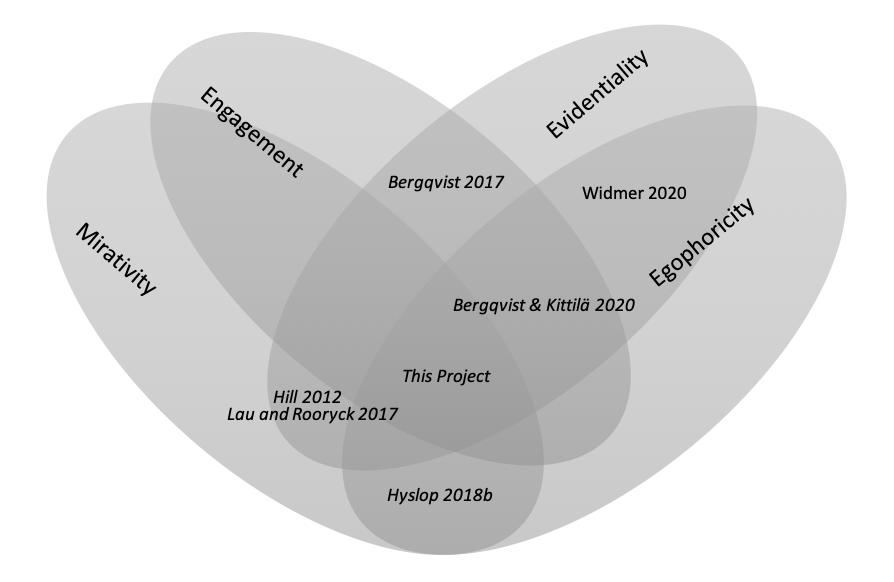
\includegraphics[width=\textwidth]{LitVenn.png}
    \caption{Examples of publications examining the crossovers between phenomena}
    \label{fig:LitVenn}
\end{figure}
